\section{Introduction}
\label{sec:Introduction}

In the Standard Model (SM) of particle physics, \CP violation is generated by a single phase in the CKM mixing matrix~\cite{Cabibbo:1963yz,doi:10.1143/PTP.49.652}.
The unitarity of this matrix leads to the condition $V_{ud}V^{*}_{ub} + V_{cd}V^{*}_{cb} + V_{td}V^{*}_{tb} = 0$, with the complex elements of the CKM matrix $V_{ij}$. 
This condition represents a triangle equation in the complex plane, where the sites define the CKM angles $\alpha$, $\beta$ and $\gamma$ 
and the area can be related to the amount of \CP violation introduced in the quark sector~\cite{Jarlskog:1985ht}.
The angle $\gamma \equiv \text{arg}[-(V_{ud}V_{ub}^{*})/(V_{cd}V_{cb}^{*})]$ is the least well-known angle of the CKM unitary triangle.
Its current world average is dominated by a combination of \lhcb measurements, obtained from several analysis of neutral $\Bs$, $\Bz$ and charged $\Bp$ decays~\cite{LHCb-CONF-2018-002}.
The value of $\gamma$ obtained from tree-level processes is an important benchmark of the SM, 
since its comparison with $\gamma$ obtained from indirect (loop-level) measurements provides a consistency check of the picture of \CP violation in the SM.\newline
In $\Bs\to\Ds\kaon\pion\pion$ decays\footnote{Throughout the document if not stated otherwise, both charge combinations of $\Bs\to\Dspm\Kpm\pion\pion$ are implied.}, sensitivity to the weak phase results from the
interference between $\bquark\to\cquark$ and $\bquark\to\uquark$  transitions achieved through $\Bs-\Bsb$ mixing \cite{Fleischer:2003yb,DeBruyn:2012jp}.
The amplitudes for both processes are of the same order in the Wolfenstein parameters $\lambda$, $\mathcal O(\lambda^3)$, so that interference effects are expected to be large.
Due to the interference between mixing and decay amplitudes, the physical \CP violating observables in these decays are functions of a combination of $\gamma$ and the mixing phase $\beta_s$, namely $\gamma - 2\beta_s$.
A time-dependent measurement of the physical quantities in this channel can therefore be interpreted in terms of either $\gamma$ or $\beta_{s}$, using the other parameter as input.
Previous measurements have been performed by the BaBar~\cite{c8cd5292565f4e2484952d2fc69f4e07,Aubert:2006tw} and Belle~\cite{Ronga:2006hv,Bahinipati:2011yq} collaborations using $\Bz\to\Dpm^{(*)}\pi^{\pm}$ decays, 
where the ratio of the interfering $\bquark\to\uquark$ and $\bquark\to\cquark$ transitions are small, limiting the sensitivity to $\gamma$.\newline
The leading order Feynman diagrams of the $\Bs\to\Ds\kaon\pion\pion$ decay are shown in Fig.~\ref{fig:decay_feynman}.
This paper presents the first measurement of the CKM angle $\gamma \equiv \text{arg}[-(V_{ud}V_{ub}^{*})/(V_{cd}V_{cb}^{*})]$ using this $\Bs$ decay channel,
where the $\kaon\pion\pion$ subsystem is dominated by excited kaon states such as the $K_{1}(1270)$ and $K_{1}(1400)$ resonances~\cite{LHCb-PAPER-2016-013}.
The branching ration of this decay mode was measured by LHCb to be
$\frac{\mathcal B(\Bs\to\Ds\kaon\pi\pi)}{\mathcal B(\Bs\to\Ds\pion\pi\pi)} = 0.052 \pm 0.005 (\text{stat}) \pm 0.003 (\text{syst})$~\cite{LHCb-PAPER-2016-013}.
The decays are analyzed using a data set corresponding to an integrated luminosity of 7.0 $\invfb$ pf $pp$ collisions recorded with the \lhcb detector at $\sqs = 7,\mbox{ } 8 \text{and} 13 \tev$ in the years 2011, 2012 and 2015-2017.


\begin{figure}[h]
\centering
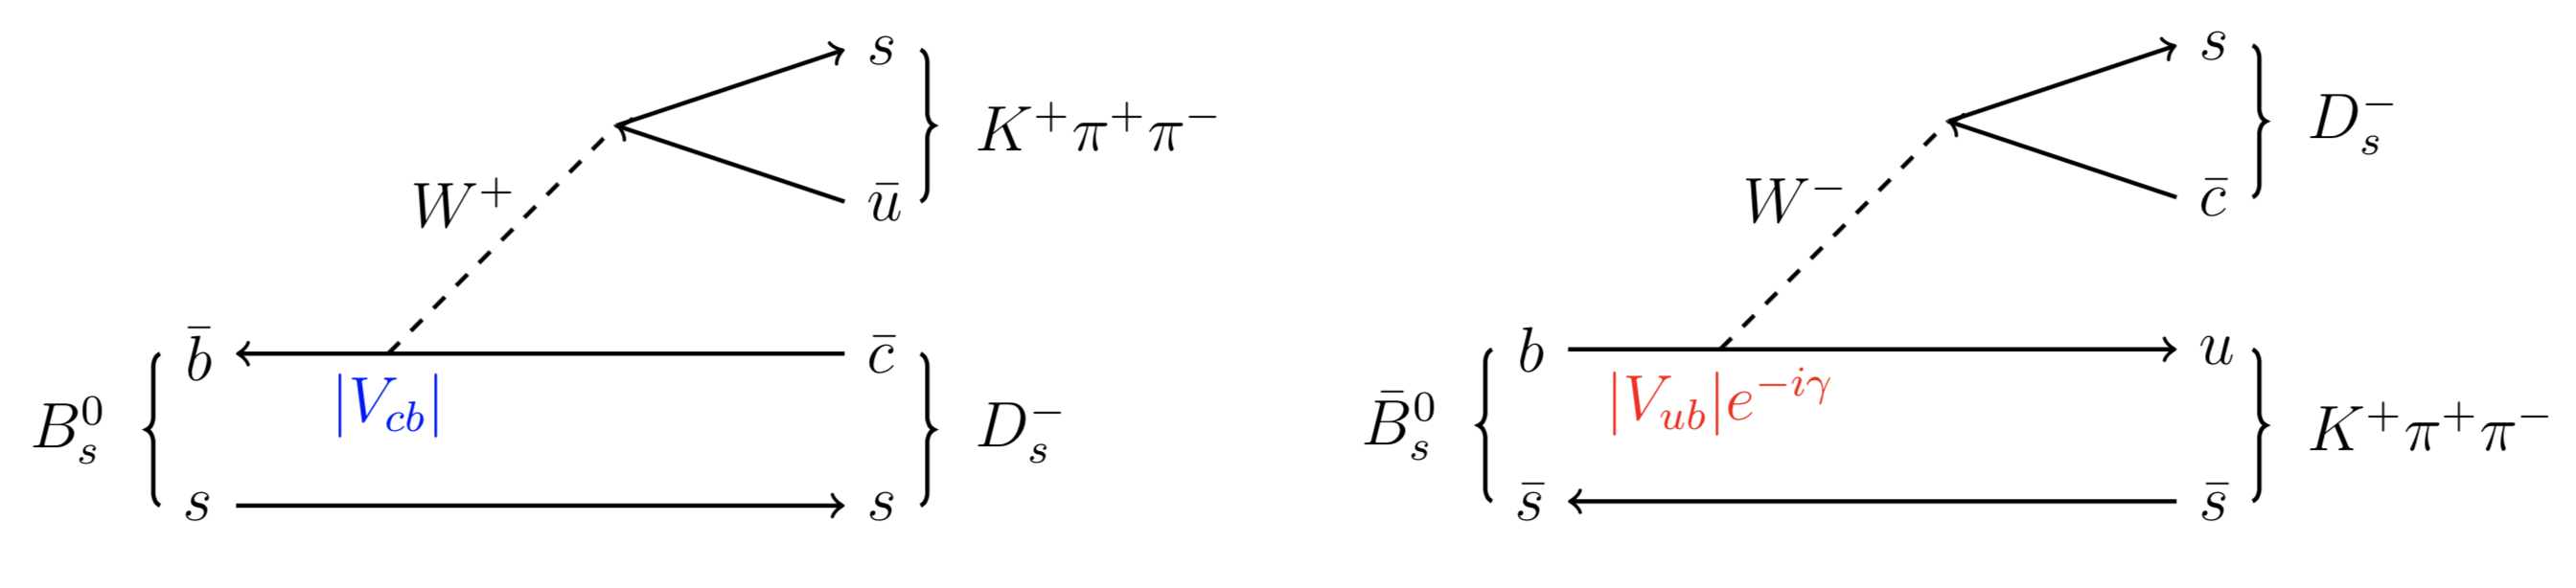
\includegraphics[height=!,width=\textwidth]{figs/feynman.png}
\caption{Feynman diagram for $B_s^0/\bar B_s^0 \to D_s^- K^+ \pip \pim$ decays.}
\label{fig:decay_feynman}
\end{figure}


\subsection{Decay rates, amplitudes and CP-violating parameters}
\label{subsec:DecRates}

The differential decay rate of $\Bs$ or $\Bsb$ decays to the final state $D_s^{-} \Kp \pi\pi$ or $D_s^{+} \Km \pi\pi$
is given by:
\begin{equation}
\begin{split}
\label{eq:PDF_full}
%       P(x,t,q_t,q_f) &\propto  [
        \frac{ \text{d}\Gamma(x,t,q,f)}{ e^{- \Gamma_s t} \, \text{d}t \, \text{d}\Phi_4} &\propto  
         \left( \vert \mathcal A^c_{f}(x) \vert^2 + \vert \mathcal A^u_{f}(x) \vert^2 \right) \, \text{cosh} \left( \frac{\Delta \Gamma_s \, t}{2}\right) \\
         & + q \, f \,  \left( \vert \mathcal A^c_{f}(x) \vert^2 - \vert \mathcal A^u_{f}(x)  \vert^2 \right) \, \text{cos} \left(\Delta m_s \, t \right)  \\
         & -2 \text{Re}\left( \mathcal A^c_{f}(x)^{*}  \, \mathcal A^u_{f}(x)  \, e^{-i f (\gamma - 2\beta_s)}  \right) \, \text{sinh} \left( \frac{\Delta \Gamma_s \, t}{2}\right)  \\
         & -2 \, q \, f \, \text{Im}\left( \mathcal A^c_{f}(x)^{*} \, \mathcal A^u_{f}(x)  \, e^{-i f (\gamma - 2\beta_s)}  \right)\, \text{sin} \left(\Delta m_s \, t \right)  
\end{split}
\end{equation}
where $q = +1$ (-1) refers to an initially produced $\Bs$ ($\Bsb$) flavour eigenstate, $q = 0$ to an undetermined initial flavour,
$f$ = +1  or -1 denotes $D_s^{-} \Kp \pi\pi$ or $D_s^{+} \Km \pi\pi$ final states and $\Gs$, $\DGs$ and $\dms$ are the width average, 
the width difference and the mass difference of the two $\Bs$ mass eigenstates $\ket{B_{L}}$ and $\ket{B_{H}}$ and $x$
represents a unique set of kinematic conditions within the five-dimensional phase space of the decay.
In this context, $\text{d}\Phi_{4}(x)$ is the element of the phase space density.
We choose a convention in which $\Delta\Gamma_s < 0$ and $\Delta m_s > 0$.
We further assume $\vert q/p \vert = 1$ for the complex coefficients $p$ and $q$ which relate the $B_s$ meson mass eigenstates to the flavour eigenstates (no \CP violation in the mixing), 
in agreement with current measurements~\cite{LHCb-PAPER-2016-013}.\newline
The static total decay amplitudes  $\mathcal A^c_{f}(x)$  and $ \mathcal A^u_{f}(x)$ are given by 
the coherent sum over all intermediate state amplitudes $A_i(x)$, each weighted by a complex coefficient,
 \begin{align}
 \mathcal A(B_s^0 \to D_s^{-} K^{+} \pi\pi) &\equiv \mathcal{A}^c_f(x) = \sum_i a^c_i \, A_i(x)   \\
 \mathcal A(\bar B_s^0 \to D_s^{-} K^{+} \pi\pi) &\equiv \mathcal A^u_f(x)  =  \sum_i  a^u_i \, A_i(x)   
% \\
 \end{align}
where the superscript $c$ ($u$) indicates a $b \to c$ ($b\to u$) quark-level transition
and $x$ represents a unique set of kinematic conditions within the five-dimensional phase space of the decay.
Assuming there is no direct \CP violation in the $\Bs$ decay implies for the $\CP$ conjugate transition amplitudes, 
$\mathcal A(\bar B_s^0 \to \bar f) =  \mathcal A^c_{\bar f}(x) = \mathcal A^c_f(\bar{x})$ and 
$\mathcal A(B_s^0 \to \bar f) = \mathcal A^u_{\bar f}(x)  = \mathcal A^u_{f}(\bar{x})$ holds.\newline
For a model-independent measurement, the differential decay rate can be integrated over the phase-space:
\begin{align}
\label{eq:PDF_intX}
        \nonumber
        \int \frac{\text{d}\Gamma(x,t,q,f)}{e^{- \Gamma_s t} \, \text{d}t \,  \text{d}\Phi_4}  \, \text{d}\Phi_4 &\propto    
        \, \text{cosh} \left( \frac{\Delta \Gamma_s \, t}{2}\right) 
          + q \, f \, C_{f} \, \text{cos} \left( \Delta m_s \, t \right)   \\
         & +  A^{\DG}_{f} \, \text{sinh} \left( \frac{\Delta \Gamma_s \, t}{2}\right)  
          - q  \, S_{f}\, \text{sin} \left(\Delta m_s \, t \right)  
\end{align}
where the following. common convention for the \CP coefficients is used:
\begin{align}
\label{eq:CPcoeff}
        C_{f}= & \frac{1-r^2}{1+r^2}   \\
        A^{\DG}_{f} = &  -\frac{2 \, r \, \kappa \, \text{cos}\left(\delta-q_f \, (\gamma-2\beta_s)\right)}{1+r^2}   \\
        S_{f} = & \,  f \, \frac{2 \, r \, \kappa \, \text{sin}\left(\delta-q_f \, (\gamma-2\beta_s)\right)}{1+r^2}   
\end{align}
The coherence factor $\kappa$, the strong phase difference $\delta$ and the ratio of the suppressed ($\bquark\to\uquark$) over favored ($\bquark\to\cquark$) decay mode, 
averaged over the phase-space, are defined as:
\begin{align}
\label{eq:coherenceFactor}
        \kappa \, e^{i\delta} &\equiv \, \frac{\int \mathcal A^c_f(x)^{*} \, \mathcal A^u_f(x)  \, \text{d}\Phi_{4}}{\sqrt{\int \vert \mathcal A^c_f(x) \vert^2 \, 
\text{d}\Phi_{4}} \sqrt{\int \vert \mathcal A^u_f(x) \vert^2 \, \text{d}\Phi_{4}}  } \\
        r &\equiv \, \frac{\sqrt{\int \vert \mathcal A^u_f(x)\vert^2 \, \text{d}\Phi_{4} }}{\sqrt{\int \vert \mathcal A^c_f(x)\vert^2 \, \text{d}\Phi_{4}}} .
\end{align}
The coherence factor dilutes the sensitivity to the weak phase $\gamma$ due to the integration over the interfering amplitudes across the phase space.
Therefore, its value is bounded between zero and unity.
The latter corresponds to the limit of only one contributing intermediate state in which case the maximum available sensitivity is reached,
while $\kappa = 0$ would result in no sensitivity to $\gamma$ at all.


\subsection{Analysis strategy}
\label{subsec:AnaStrat}

The analysis strategy follows a two-stage procedure. 
After the selection of signal candidates, a unbinned maximum likelihood fit is performed to the invariant mass distribution of $\Bs$ candidates, 
in order to seperate the signal $\Bs\to\Ds\kaon\pion\pion$ candidates from various backgrounds.
Using the information from this fit, the sPlot technique~\cite{Pivk:2004ty} is used to statistically subtract the background from the data sample.
At the second stage, the CP-violating parameters, as well as the CKM angle $\gamma$, are determined from a time-dependent fit to the background-subtracted signal sample. 
Two seperate measurements are performed at this stage:\newline
To account for the non-constant strong phase across the phase-space, a time-dependent amplitude fit is performed, 
where $\gamma$ can directly be determined in the fit using a suitable amplitude model and external input for the weak mixing angle $\beta_{s}$; \newline
A coherence factor is introduced  as additional hadronic parameter to the decay-time dependent, phase-space averaged fit. 
In this fit, the CP-violating parameters, defined in Section~\ref{subsec:DecRates} are determined and can be used to calculate $\gamma$, using $\beta_{s}$ as an input to the measurement.\newline
The topologically very similar, yet flavour specific decay $\Bs\to\Ds\pion\pion\pion$ is used as calibration channel,
not only to calibrate the tagging algorithms and determine the decay-time acceptance, but also to constrain the $\Bs-\Bsb$ mixing frequency.
The decay-time resolution is determined using a data driven technique, exploiting promptly produced $\Ds$ mesons.


